\section{Cross teams process}
In the beginning of the semester, all groups had to define the process for \gls{G19}. 
This resulted in a manual\cite{processManual}, written by \gls{POT}, defining the practices and process to be followed by the groups. The decisions described in the following, are defined in the manual. 

Overall, the teams are organized as \Glspl{fullStack}. A \gls{fullStack}. This means, that the teams work on full user stories rather than on a specific areas. 
This was chosen, because students from earlier years expressed that they have had a lot of problems working in specific areas\cite{fullStackVSSpecific}.

To make sure all \glspl{devTeam} get the required knowledge in the specific areas, there are dedicated \glspl{skillGroup}. There are a member from each group in every \gls{skillGroup}, and these members are expected to have knowledge about a specific area of the system. 

The \gls{G19} process uses a technique called \gls{SOS}. This is a technique for running a Scrum process in bigger teams and is adapted to fit the needs of \gls{G19}. 
The activities resembles the normal Scrum activities, but instead of \gls{devTeam} having their own product backloc and activities in the group, each group is seen as something similar to  are adapted to fit multiple \glspl{devTeam} working together. There are planned a total of four sprints, and in the following is described the activities in each sprint:

\begin{itemize}
    \item \Gls{SOSSprintPlanning}
    \item \Gls{SOSStandUp}
    \item \Gls{skillGroup} Meetings
    \item \Gls{ReleasePreparation}
    \item \Gls{SOSSprintRetrospective}
    \item \Gls{SOSSprintReview}
    \item Release Party
\end{itemize}

The SOS process is graphically represented in \autoref{fig:SOSProcess}. Here, the circles represent an activity. The stickmen represents a group member with a role. The "any member" role represents all of the group members. If when one stickman is placed in an activity, it means that one person from the group has to attend. 
One of each \gls{skillGroup} charecters are placed in the \gls{skillGroup} meeting activity. That means that it is them that attends the \gls{skillGroup} meetings.
When no stickman is placed in an activity, that means, that the activity is for everybody. 
The activities are ordered chronologically. Activities placed on the loop are repeated.

\begin{figure}[h]
    \begin{center}
        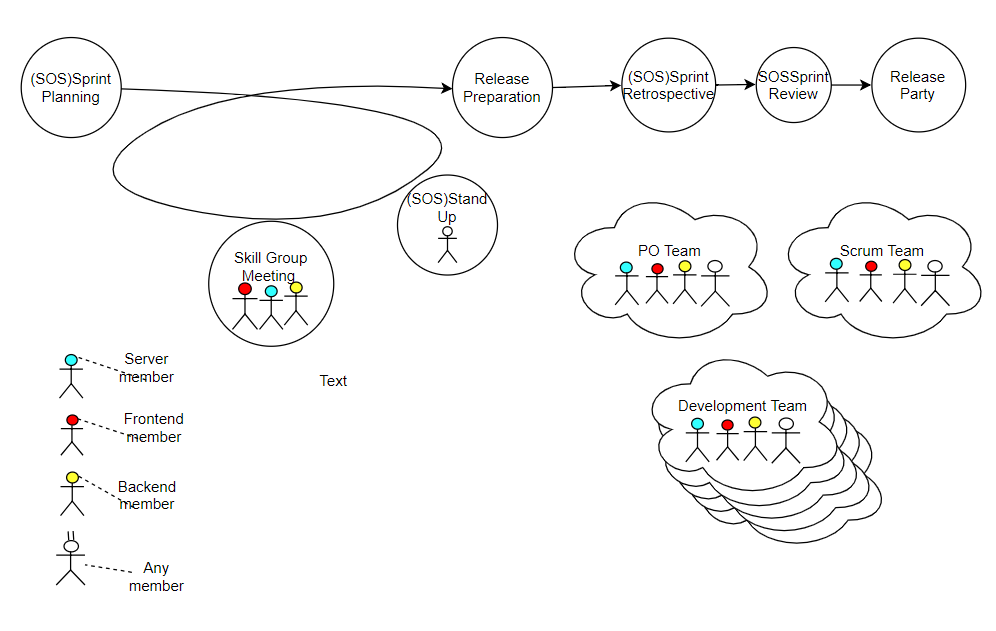
\includegraphics[width=0.95\textwidth]{figures/SOSProcess}
    \end{center}
    \caption{Representation of the \gls{SOS} process.}
    \label{fig:SOSProcess}
\end{figure}

The seven groups are represented with a cloud. \gls{SOS} only describes the process between \glspl{devTeam}. It is up to each group to define their own process, as long as it fits within the \gls{SOS} guidelines. 

The following part will contain a description of each of the activities.

\Gls{SOSSprintPlanning} is a meeting held on the first day of each sprint. All members of \Gls{G19} attends. Before the \Gls{SOSSprintPlanning}, the \gls{POT} has prepared user stories for the sprint backlog, and the purpose of the sprint. 
This is then presented for all \glspl{devTeam}, and the teams will then choose which user stories to implement, and estimate the chosen stories. 
The members of the \gls{POT} is available for questions, and needs to accept the other groups chosen stories and estimates. 
When the \glspl{devTeam} has found a number of tasks appropriate for them, they should leave the meeting. 
 
\Gls{SOSStandUp} is a meeting that is held one to three times a week. The purpose of this meeting, is to share the progress and challenges between the groups, so 